%!TEX root = ../report.tex
\documentclass[../report.tex]{subfiles}
\begin{document}
    \chapter{Evaluation and Results}\label{ch_eval}
        \noindent
	This chapter presents the results of experiments whose implementation details were provided in the last chapter. Besides, the outcomes are systematically analyzed and evaluated.
	
	
	\section{Background}
	\noindent
	We conducted the first three experiments (A. patient-wise attribution map generation, B. composite face generation, and C. syndrome-wise attribution map generation) on each of the 139 frequent syndrome classes in the GMDB dataset. However, as mentioned earlier, experimental artifacts related to six of the syndromes (CDLS, WBS,  CSS,  NBS, HPMRS and SMOS) were evaluated by an experienced clinical geneticist. The clinician specialized in the diagnosis of three of the syndromes (CDLS, WBS, HPMRS) and had less familiarity with others. Therefore, analyses and discussions on experimental results mostly revolve around the three syndrome categories. Besides, some important findings from other syndromes are also provided. In this section, some background information regarding facial phenotypic features of the syndromes discussed in this chapter is given. 
	
	\subsubsection{Cornelia De Lange Syndrome}
	Cornelia de Lange syndrome (CDLS) is a rare genetic condition present at birth. Multiple physical and intellectual abnormalities characterize it. There are different variants of the syndrome, each identified with its own set of facial features. However, the profile of eyebrows is predominantly considered for diagnosing the syndrome. Figures \ref{fig_cdls_char} and \ref{fig_cdls} show samples contain other facial features related to the genetic condition.
		\begin{figure}[H]
		\centering
		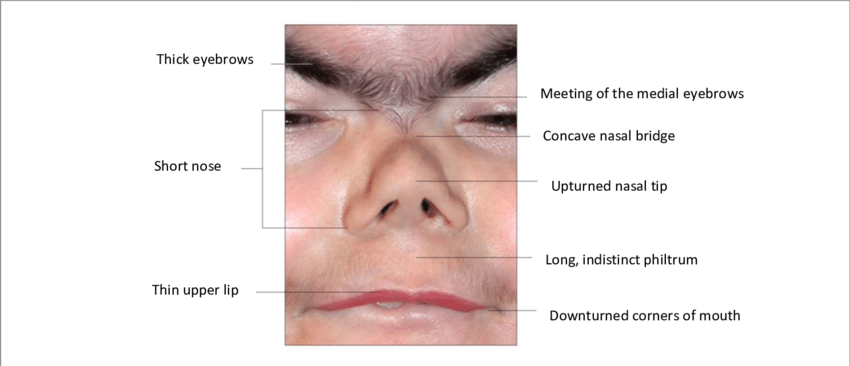
\includegraphics[scale=0.5, trim = 1cm 1cm 1cm 1cm, clip]{chapter6/cdls/cdls_ref.png}	
		\caption[Cardinal features of CDLS]{Cardinal facial features of CDLS. Image source: \cite{kline2018diagnosis}}
		\label{fig_cdls_char}
	\end{figure}
	
	\begin{figure}[H]
		\centering
		\begin{subfigure}[t]{0.24\textwidth}
			\centering
			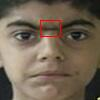
\includegraphics[width=\textwidth]{chapter6/cdls/0_3529.jpg}
			\caption{Synophrys}
		\end{subfigure}
		\begin{subfigure}[t]{0.24\textwidth}
			\centering
			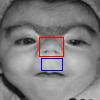
\includegraphics[width=\textwidth]{chapter6/cdls/9_2000.jpg}
			\caption{Depressed nasal bridge (red), long philtrum (blue)}
		\end{subfigure}	
		\begin{subfigure}[t]{0.24\textwidth}
			\centering
			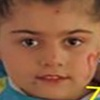
\includegraphics[width=\textwidth]{chapter6/cdls/33_3580.jpg}
			\caption{Thin upper lip}
		\end{subfigure}	
		\begin{subfigure}[t]{0.24\textwidth}
			\centering
			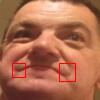
\includegraphics[width=\textwidth]{chapter6/cdls/117_3699.jpg}
			\caption{Down-turned corners of mouth}
		\end{subfigure}
		\caption[Instances of CDLS from GMDB dataset]{Instances of CDLS from GMDB dataset annotated with phenotypic facial features}
		\label{fig_cdls}
	\end{figure}
	
	\subsubsection{Williams Beuren Syndrome}
	Williams Beuren Syndrome (WBS) or Williams syndrome is a rare genetic condition that affects many parts of the human body. The disorder is marked by both prenatal (before birth) and postnatal growth retardation. A flat midface, long philtrum, and thick lips are some characteristic facial features associated with the syndrome. Refer to figures \ref{fig_williams_char} and \ref{fig_wil_gmdb} contain an animated representative face and examples from the GMDB dataset, respectively. 
	\begin{figure}[H]
	\centering
	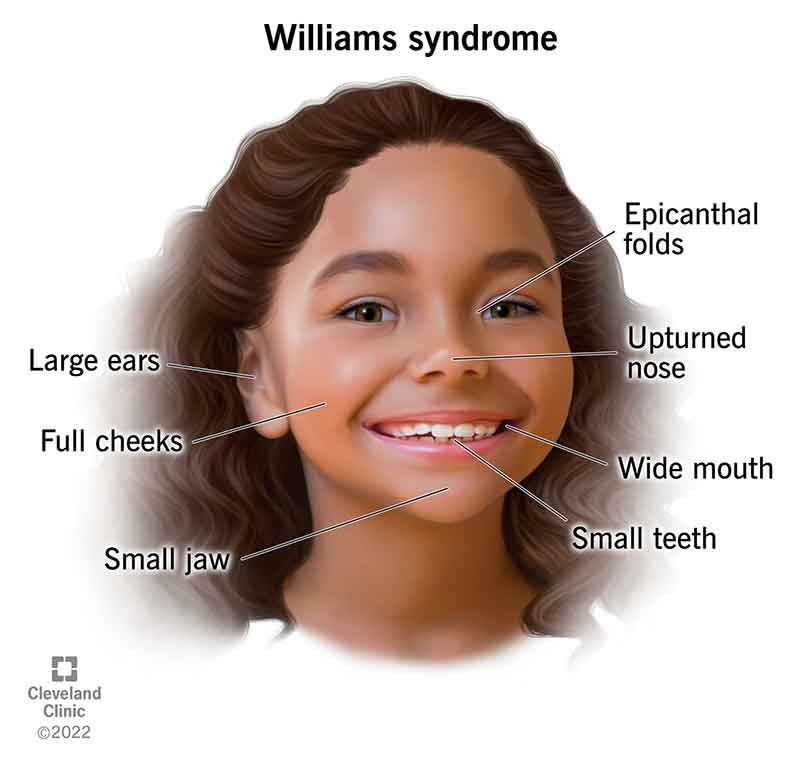
\includegraphics[scale=0.2]{chapter6/william/williams_syndrome_ref.jpg}	
	\caption[An animated characteristic face of WBS]{An animated characteristic face of WBS. Image source: Cleveland clinic \protect\footnotemark.}
	\label{fig_williams_char} 
	\end{figure}
	 \footnotetext{Cleveland clinic - \url{https://my.clevelandclinic.org/health/diseases/15174-williams-syndrome}}
	\begin{figure}[H]
		\centering
		\begin{subfigure}[t]{0.24\textwidth}
			\centering
			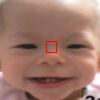
\includegraphics[width=\textwidth]{chapter6/william/4_37.jpg}
			\caption{Depressed nasal bridge}
		\end{subfigure}
		\begin{subfigure}[t]{0.24\textwidth}
			\centering
			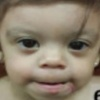
\includegraphics[width=\textwidth]{chapter6/william/4_73.jpg}
			\caption{Long philtrum}
		\end{subfigure}	
			\begin{subfigure}[t]{0.24\textwidth}
			\centering
			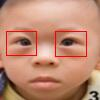
\includegraphics[width=\textwidth]{chapter6/william/130_36.jpg}
			\caption{Puffy eyes}
		\end{subfigure}	
			\begin{subfigure}[t]{0.24\textwidth}
			\centering
			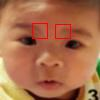
\includegraphics[width=\textwidth]{chapter6/william/164_35.jpg}
			\caption{Medial eyebrow flares}
		\end{subfigure}	
	\caption[Instances of WBS from GMDB dataset]{Instances of WBS from GMDB dataset annotated with phenotypic facial features}
	\label{fig_wil_gmdb}
	\end{figure}

	\subsubsection{Hyperphosphatasia with Mental Retardation Syndrome}
	Hyperphosphatasia with intellectual disability or mental retardation syndrome (HPMRS)  is characterized by intellectual diability, seizures, facial dysmorphism and other abnormalities. The syndrome occurs in multiple variants. Some facial features linked to HPMRS1 include hypertelorism, short philtrum, short nose, broad nasal tip, broad nasal bridge, long palpebral fissures, and upslanting palpebral fissures.
	 \begin{figure}[H]\label{fig_hpmrs}
	 	\centering
	 	\begin{subfigure}[t]{0.17\textwidth}
	 		\centering
	 		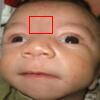
\includegraphics[width=\textwidth]{chapter6/hpmrs/2_499.jpg}
	 		\caption{Hypertelorism}
	 	\end{subfigure}
	 	\begin{subfigure}[t]{0.17\textwidth}
	 		\centering
	 		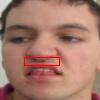
\includegraphics[width=\textwidth]{chapter6/hpmrs/15_1758.jpg}
	 		\caption{Short philtrum}
	 	\end{subfigure}	
	 	\begin{subfigure}[t]{0.17\textwidth}
	 		\centering
	 		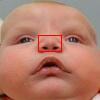
\includegraphics[width=\textwidth]{chapter6/hpmrs/17_1774.jpg}
			\caption{Short nose}
	 	\end{subfigure}	
	 	\begin{subfigure}[t]{0.17\textwidth}
	 		\centering
	 		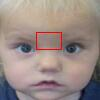
\includegraphics[width=\textwidth]{chapter6/hpmrs/20_888.jpg}
	 		\caption{Broad nasal bridge}
	 	\end{subfigure}	
	 	\begin{subfigure}[t]{0.17\textwidth}
	 		\centering
	 		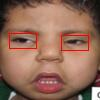
\includegraphics[width=\textwidth]{chapter6/hpmrs/33_1773.jpg}
	 		\caption{Upslanting palpebral fissures}
	 	\end{subfigure}	
	 	\caption[Instances of HPMRS from GMDB dataset]{Instances of HPMRS from GMDB dataset annotated with phenotypic facial features}
	 \end{figure}
	 
	 \subsubsection{Coffin Siris Syndrome}
	 	Coffin Siris syndrome (CSS) is a congenital (may be evident at birth) rare genetic condition that affects multiple body systems. This syndrome also occurs in multiple variants. CSS 1 is characterized by the following facial features: short philtrum, thin upper-lip vermilion, and thick lower-lip vermilion, small chin, broad nasal tip, down-slanting palpebral fissures, bushy eyebrows, long eyelashes, large mouth, lower lip droop, and broad nasal tip.
	 \begin{figure}[H]\label{fig_cfs}
	 	\centering
	 	\begin{subfigure}[t]{0.17\textwidth}
	 		\centering
	 		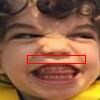
\includegraphics[width=\textwidth]{chapter6/cfs/5_1981.jpg}
	 		\caption{Short philtrum}
	 	\end{subfigure}
	 	\begin{subfigure}[t]{0.17\textwidth}
	 		\centering
	 		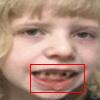
\includegraphics[width=\textwidth]{chapter6/cfs/6_810.jpg}
	 		\caption{Thin upper-lip vermilion and thick lower-lip vermilion }
	 	\end{subfigure}	
	 	\begin{subfigure}[t]{0.17\textwidth}
	 		\centering
	 		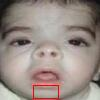
\includegraphics[width=\textwidth]{chapter6/cfs/17_2539.jpg}
	 		\caption{Small chin}
	 	\end{subfigure}	
	 	\begin{subfigure}[t]{0.17\textwidth}
	 		\centering
	 		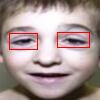
\includegraphics[width=\textwidth]{chapter6/cfs/20_2465.jpg}
	 		\caption{Downslanting palpebral fissures}
	 	\end{subfigure}	
	 	\begin{subfigure}[t]{0.17\textwidth}
	 		\centering
	 		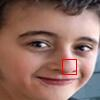
\includegraphics[width=\textwidth]{chapter6/cfs/46_1986.jpg}
	 		\caption{Broad nasal tip}
	 	\end{subfigure}	
	 	\caption[Instances of CSS from GMDB dataset]{Instances of CSS from GMDB dataset annotated with phenotypic facial features}
	 \end{figure}
	 
	 
    \section{Experiment A. Patient-wise Attribution Map Generation}
    \noindent
    The clinician was presented with attribution maps of 23 instances from six different syndromes classes in GMDB. However, as mentioned earlier, his specialization was limited to three syndromes which were represented by 15 samples in the questionnaire. Table \ref{tab_cl_acc} shows the sample distribution and diagnostic performance of the clinician for each syndrome class without the aid of attribution maps. As described in  Chapter \ref{ch_method}, it is important to note that only samples from the test split of GMDB that were correctly classified by the GestaltMatcher classifier model were chosen for evaluation. 
    
    
   	\begin{figure}[H]
   	\centering
   	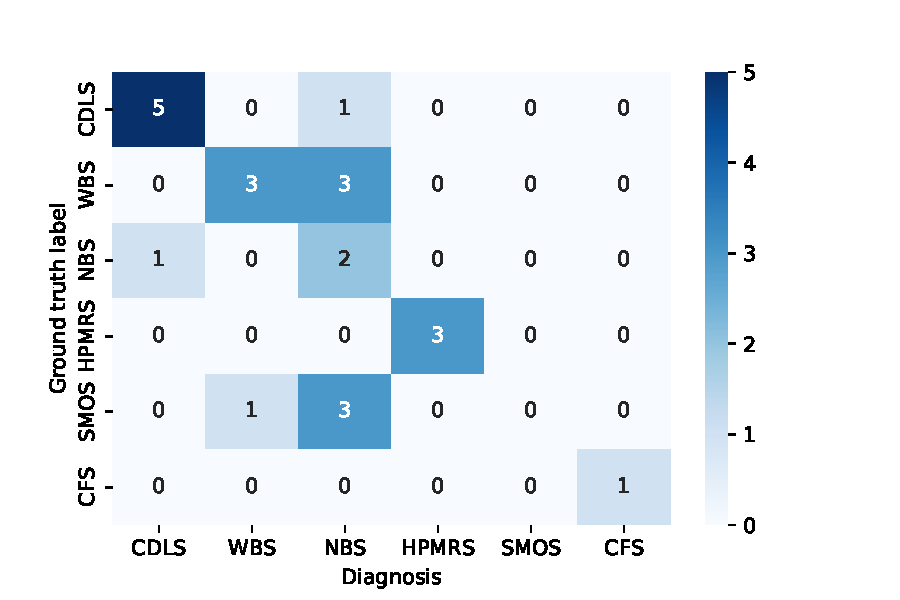
\includegraphics[scale=0.6,trim=0.5cm 0cm 0.5cm 0cm, clip]{chapter6/clinician_conf_matrix.pdf}	
   	\caption[Confusion matrix representing the clinician's
   	diagnostic performance]{Confusion matrix representing the clinician's
   	diagnostic performance}
   \label{fig_clin_perf_mtx} 
   \end{figure}
    

\begin{table}[H]
	\centering
	\begin{tabular}{|c|c|c|c|}
		\hline
		\textbf{Syndrome} & \textbf{Sample count} & \textbf{\begin{tabular}[c]{@{}c@{}}Clinician\\ specializes in \\ syndrome\end{tabular}} & \textbf{Accuracy} \\ \hline
		CDLS              & 6                     & yes                                                                                     & 0.83              \\ \hline
		WBS               & 6                     & yes                                                                                     & 0.50              \\ \hline
		NBS               & 3                     & no                                                                                      & 0.67              \\ \hline
		HPMRS             & 3                     & yes                                                                                     & 1.00              \\ \hline
		SMOS              & 4                     & no                                                                                      & 0.00              \\ \hline
		CFS               & 4                     & no                                                                                      & 1.00              \\ \hline
	\end{tabular}
\caption{Diagnostic performance of the clinician on samples in the questionnaire}
\label{tab_cl_acc}
\end{table}
 

  \subsubsection{Usefulness of Attribution Maps in Diagnoses}
  Fig \ref{fig_patient_flow} in Chapter \ref{ch_method} enumerated the following possible inferences, which can be obtained from responses in the patient-wise attribution map evaluation section of the questionnaire:
  \begin{itemize}
  	\item A. Attribution maps mislead the clinician to make an incorrect diagnosis
  	\item B. Attribution maps reinforce the clinician's correct diagnosis
  	\item C. Attribution maps help the clinician to correct his diagnosis
  	\item D. Attribution maps fail to help the clinician to correct his diagnosis
  \end{itemize} 
  Here, we describe the use of attribution maps and the performance of methods used to generate them by binning clinician responses into one of the above mentioned and analyzing them. 
  
  As shown in Figure \ref{fig_clin_perf_mtx}, the clinician correctly diagnosed 11 out of the total 15 patient images presented to him from the syndromes of his specialty without the aid of attribution maps. His responses to the subsequent questions (refer to questions 2b - 2e in Table \ref{tbl_synd_wise}) asked after the 11 correctly diagnosed cases indicate that the attribution maps reinforced correct diagnoses (scenario B) in eight cases and did not prove helpful (scenario A) in three. Within the eight occurrences of scenario B, attribution maps using FullGrad were marked to best highlight the associated facial features in five, followed by the maps of other methods in one each. Among the four misdiagnosed instances, none of the attribution maps proved effective in correcting three of his predictions (scenario D), and a FullGrad attribution map helped him correct one (scenario C). 
  To summarize, the clinician found attribution maps, in general, helpful for diagnosis in 9 out of 15 instances, and also chose FullGrad maps to highlight relevant facial features in most cases.
		\begin{figure}[H]
		\centering			
		\begin{subfigure}[t]{1\textwidth}
			\centering
			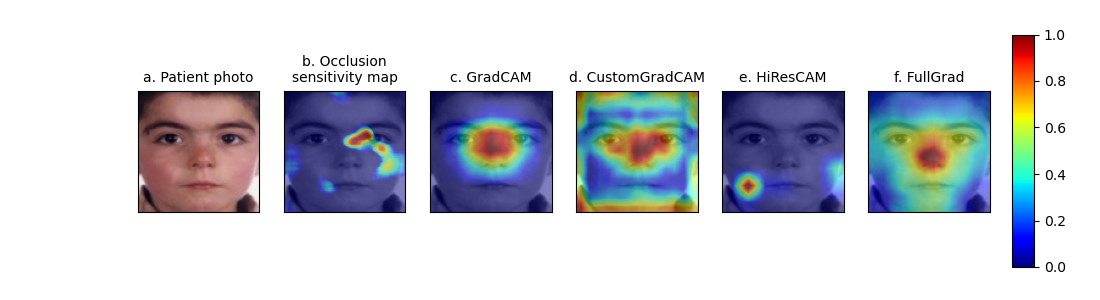
\includegraphics[width=\textwidth, trim = 1cm 2.50cm 1cm 2cm, clip]{chapter6/cdls/0_205.png}
			\caption{Patient with CDLS and eyebrows specified as the key feature}
			\label{sfig_match_1}
		\end{subfigure}
		\begin{subfigure}[t]{1\textwidth}
			\centering
			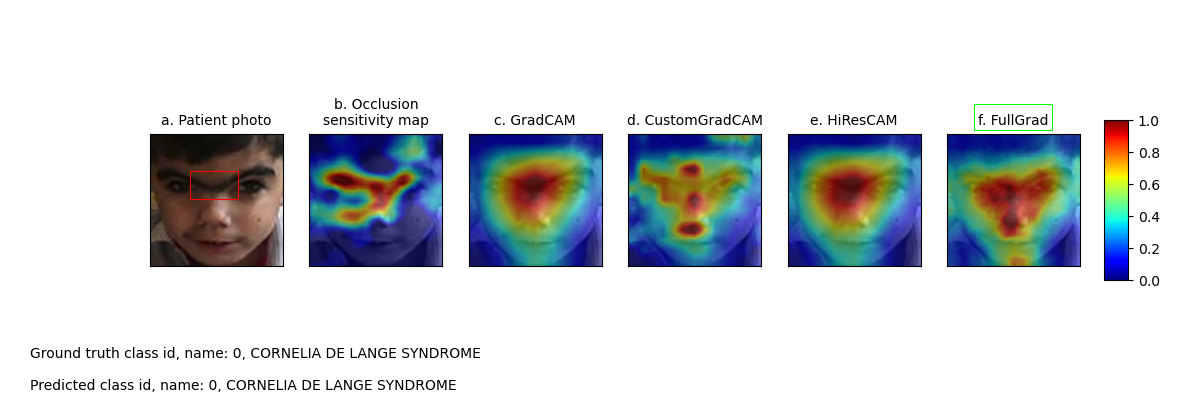
\includegraphics[width=\textwidth, trim = 1cm 2.50cm 1cm 2cm, clip]{chapter6/cdls/4_3556.png}
			\caption{Patient with CDLS and synophrys feature}
			\label{sfig_match_2}
		\end{subfigure}
		\begin{subfigure}[t]{1\textwidth}
			\centering
			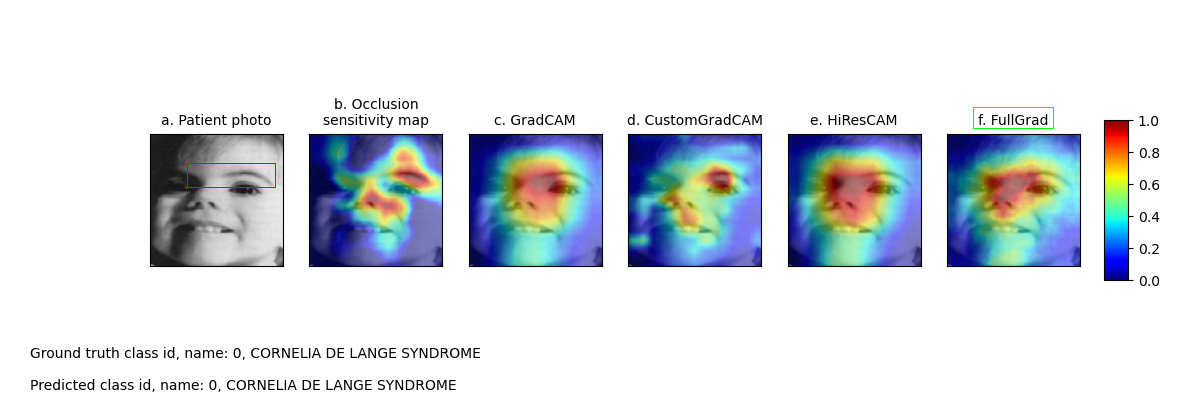
\includegraphics[width=\textwidth, trim = 1cm 2.50cm 1cm 2cm, clip]{chapter6/cdls/6_222.png}
			\caption{Patient with CDLS and eyebrows specified as the key feature}
			\label{sfig_match_3}
		\end{subfigure}
		\begin{subfigure}[t]{1\textwidth}
			\centering
			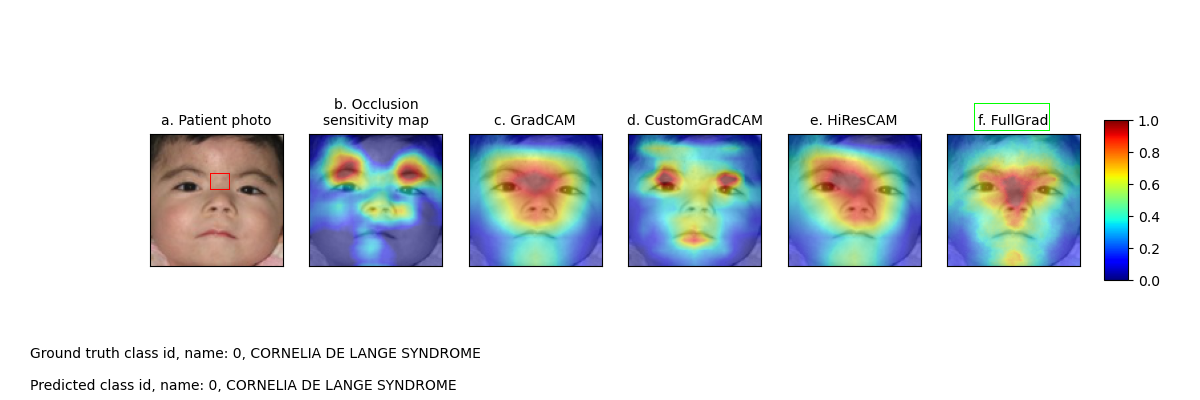
\includegraphics[width=\textwidth, trim = 1cm 2.50cm 1cm 2cm, clip]{chapter6/cdls/7_285.png}
			\caption{Patient with CDLS and nose, depressed nasal bridge reported as the key features}
			\label{sfig_match_4}
		\end{subfigure}
		\begin{subfigure}[t]{1\textwidth}
		\centering
		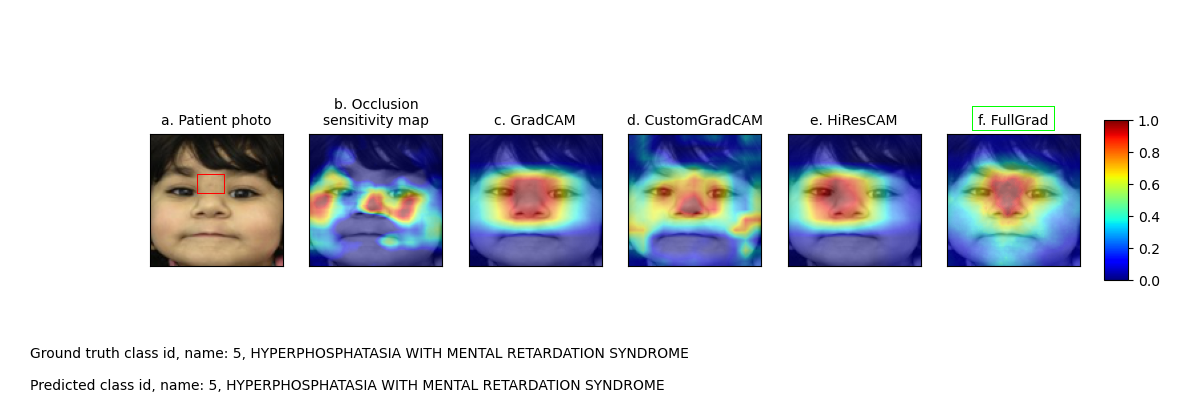
\includegraphics[width=\textwidth, trim = 1cm 2.50cm 1cm 2cm, clip]{chapter6/hpmrs/4_2442.png}
		\caption{Patient with HPMRS and nasal bridge reported as the key feature}
		\label{sfig_match_5}
		\end{subfigure}
		\caption[Attribution maps of instances in which clinician's attention regions matched that of the classifier model]{Attribution maps of instances in which clinician's attention regions matched that of the classifier model. Key features specified and methods chosen by the clinician are boxed in red and green colors respectively}
	\label{fig_match_cl_maps}
	\end{figure}
	\begin{figure}[H]
		\begin{subfigure}[t]{1\textwidth}
			\centering
			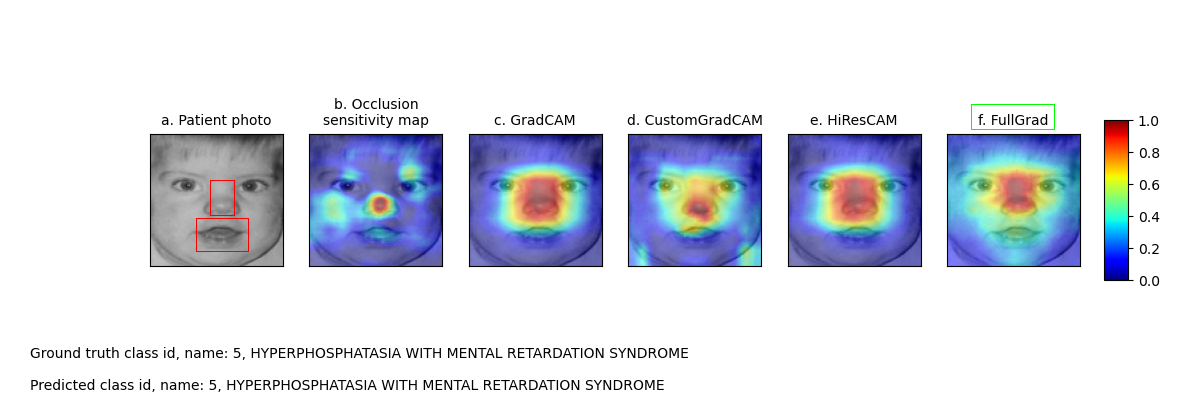
\includegraphics[width=\textwidth, trim = 1cm 2.50cm 1cm 2cm, clip]{chapter6/hpmrs/0_2425.png}
			\caption{Patient with  HPMRS, and nose and mouth specified as key features}
			\label{sfig_diff_1}
		\end{subfigure}
		\begin{subfigure}[t]{1\textwidth}
			\centering
			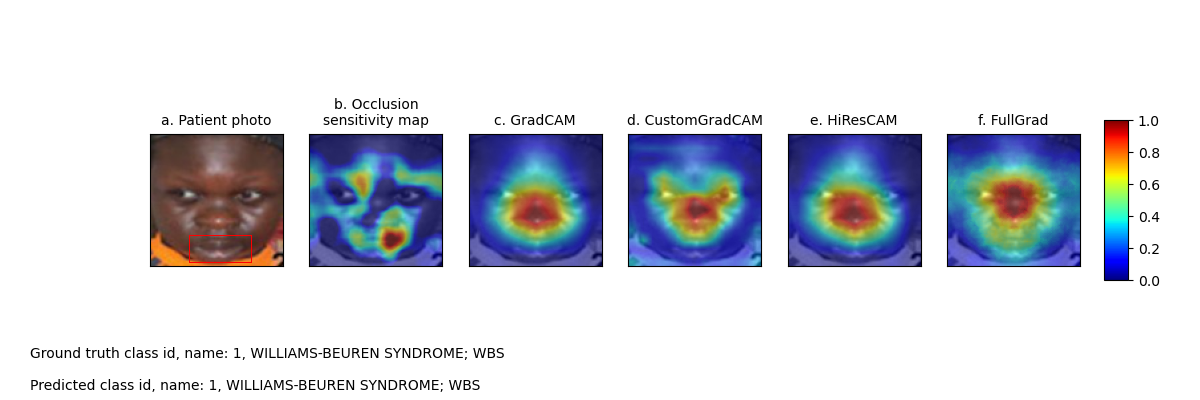
\includegraphics[width=\textwidth, trim = 1cm 2.50cm 1cm 2cm, clip]{chapter6/william/5_31.png}
			\caption{Patient with  WBS, and lips specified as the key feature}
			\label{sfig_diff_2}
		\end{subfigure}
		\begin{subfigure}[t]{1\textwidth}
		\centering
		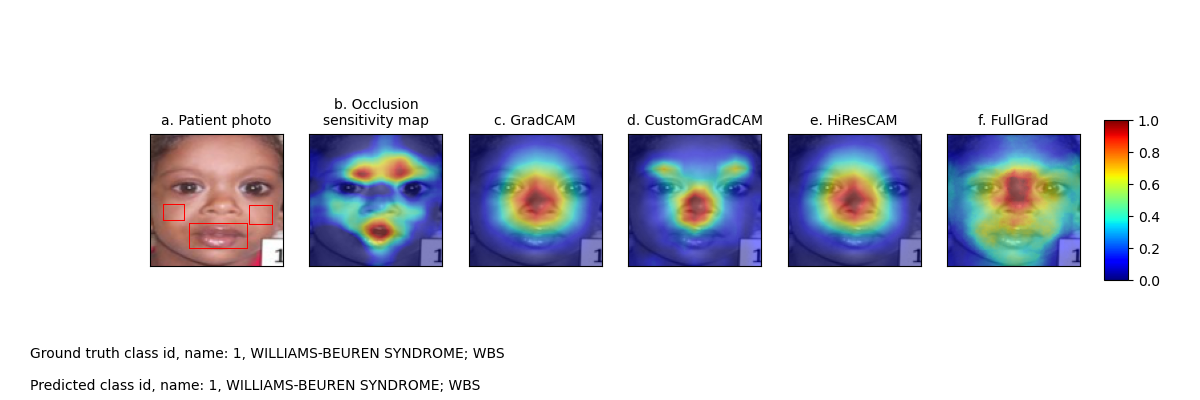
\includegraphics[width=\textwidth, trim = 1cm 2.50cm 1cm 2cm, clip]{chapter6/william/2_137.png}
		\caption{Patient with  WBS, and lips and cheeks specified as key features}
		\label{sfig_diff_3}
		\end{subfigure}
		\begin{subfigure}[t]{1\textwidth}
		\end{subfigure}
		\caption[Attribution maps of instances in which clinician's attention regions differed from that of the classifier model]{Attribution maps of instances in which clinician's attention regions differed from that of the classifier model. Key features specified by the clinician are boxed in red. Method chosen for the first instance is boxed in green color.}
		\label{fig_diff_cl_maps}
	\end{figure}
	\subsubsection{Comparing Attention Regions}
	Besides identifying syndromes and rating attribution maps, the clinician was asked to specify the key facial features he used for diagnosis (Refer to question 2b in Table \ref{tbl_synd_wise}). From his answers, let us compare his regions of attention with that of the GestaltMatcher classifier model, represented in the form of attribution maps.  Figure \ref{fig_match_cl_maps} and Figure \ref{fig_diff_cl_maps}  contain examples of attribution map sets of correctly diagnosed samples, for which features considered crucial by the clinician matched and differed with that of the classifer, respectively.
	
	He reported the eyebrow region to contain key features for diagnosing CDLS, in most of the cases, especially the occurrence of synophrys such as found in figures \ref{sfig_match_1} and \ref{sfig_match_2}. Besides, features in the nose region, such as the depressed nasal bridge (refer Figure \ref{sfig_match_5}) were also considered important for his identification. Attribution maps generated using FullGrad were reported to correctly highlight key features of CDLS in three out of six cases, followed by GradCAM in two. The clinical geneticist found none of the maps to be helpful in diagnosing one instance. On the whole, attribution maps were found to be helpful in diagnosing CDLS.\\
	In the case of HPMRS samples, nose and mouth regions were pointed out to contain the syndrome's characteristic features (refer to figures \ref{sfig_match_5} and \ref{sfig_diff_1}). FullGrad maps are reported to highlight the characteristic nose region in most cases. However, none of the maps highlighted the mouth feature, as can be observed from  Figure \ref{sfig_diff_1}.
	
    Samples presented from WBS were reported to contain key facial features in the lip and cheek regions of the face (refer to figures \ref{sfig_diff_2} and \ref{sfig_diff_3}). Analyzing clinician responses pertaining to the syndrome reveals that none of the attribution maps proved helpful for him, both in cases of reinforcing correct diagnoses and correcting misdiagnoses. More importantly, it can be observed that the maps highlighted the nose region, a feature that is not characteristic of the syndrome. However, regions highlighted in occlusion sensitivity maps contain features that the clinician considered. This finding raised doubts on faithfulness \footnote[1]{Accurate representation of the reasoning process behind a model's prediction} of the considered attribution methods. Therefore, we attempted to understand the cause of the issue by visualizing and analyzing layer-wise activation maps of different samples.
    
    \subsubsection{Layer-wise Activation Visualization and Analysis} \label{sec_layer_wise}
    We generated attribution maps for all ten convolutional layers of the classifier model using GradCAM and HiResCAM methods. This was done to check whether the missing features get highlighted in attributions of layers other than what were chosen for the experiment. We chose conv\_9 for GradCAM and HiResCAM, and conv\_6, conv\_7, and conv\_9 to generate maps using CustomGradCAM. FullGrad is a layer-agnostic approach, and therefore was excluded.
    
	Figure \ref{fig_layer_quest} contains layer-wise visualizations for samples whose attribution maps failed to highlight the key facial features. The first pair of visualizations correspond to the image in Figure \ref{sfig_diff_1} whose maps failed to highlight the mouth region. The area gets highlighted in the conv\_7 layer visualization using GradCAM. Likewise, in cases of visualizations of WBS samples (refer second and third pair of rows in Figure \ref{fig_layer_quest}), the key features in lip and cheek regions get highlighted in other convolutional layers.
	
	We extended this analysis to samples in WBS which were not included in the questionnaire. This was performed to find whether visualizations of any particular layer or set of layers highlighted key features in all instances. Figure \ref{fig_layer_gmdb} contains visualizations of three of such samples, whose key features are in the lip region. The region was found to be highlighted in visualizations of different layers in different samples. This inconsistent behavior of attribution methods poses a challenge in using them to explain GestaltMatcher predictions in a clinical setting.  
    \begin{sidewaysfigure}
    	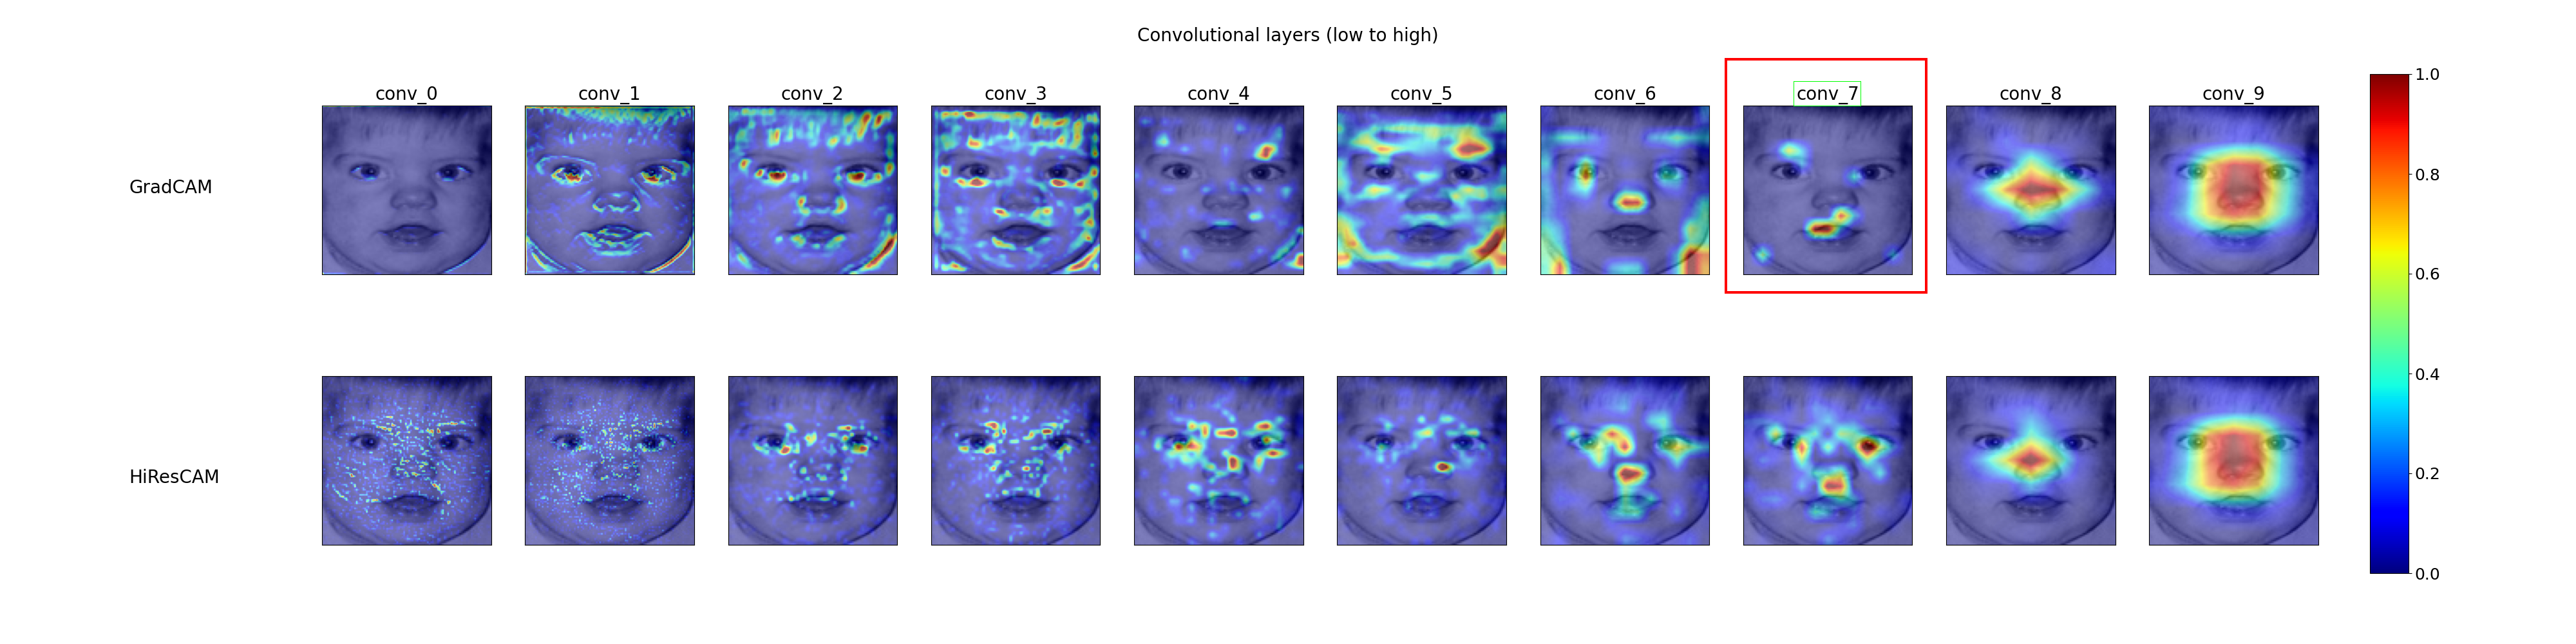
\includegraphics[scale=0.22, trim = 1cm 2cm 1cm 2cm, clip]{chapter6/hpmrs/0_2425_layer.png}
    	
    	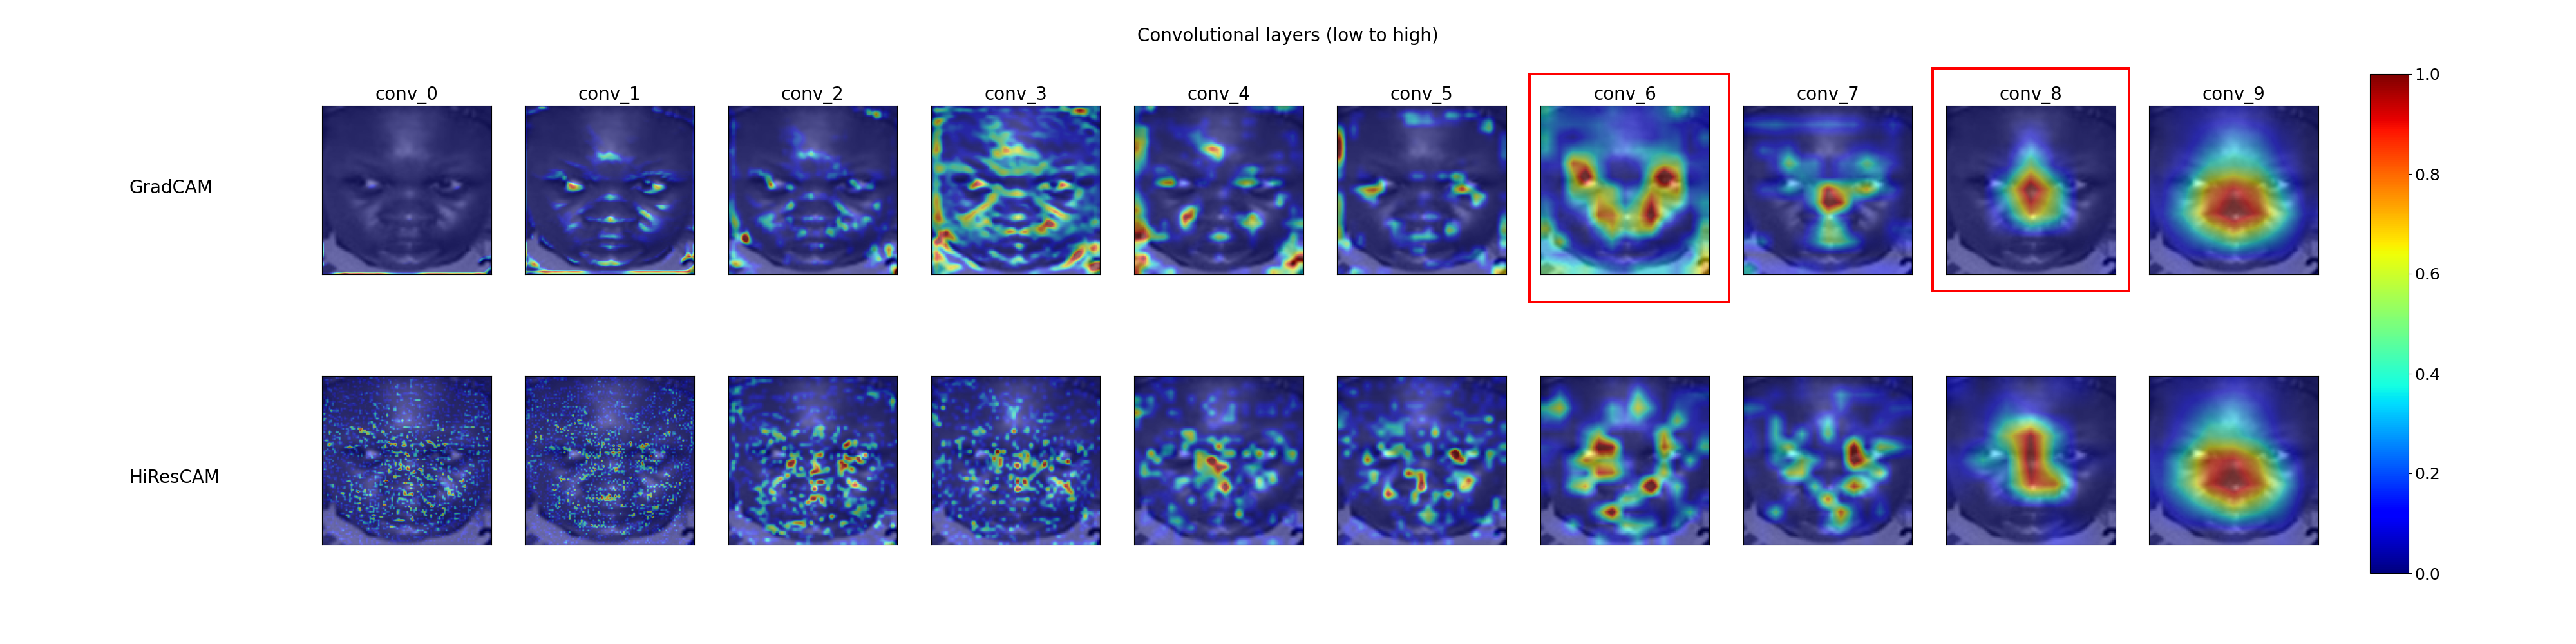
\includegraphics[scale=0.22, trim = 1cm 2.50cm 1cm 2.50cm, clip]{chapter6/william/5_31_layer.png}
	      
    	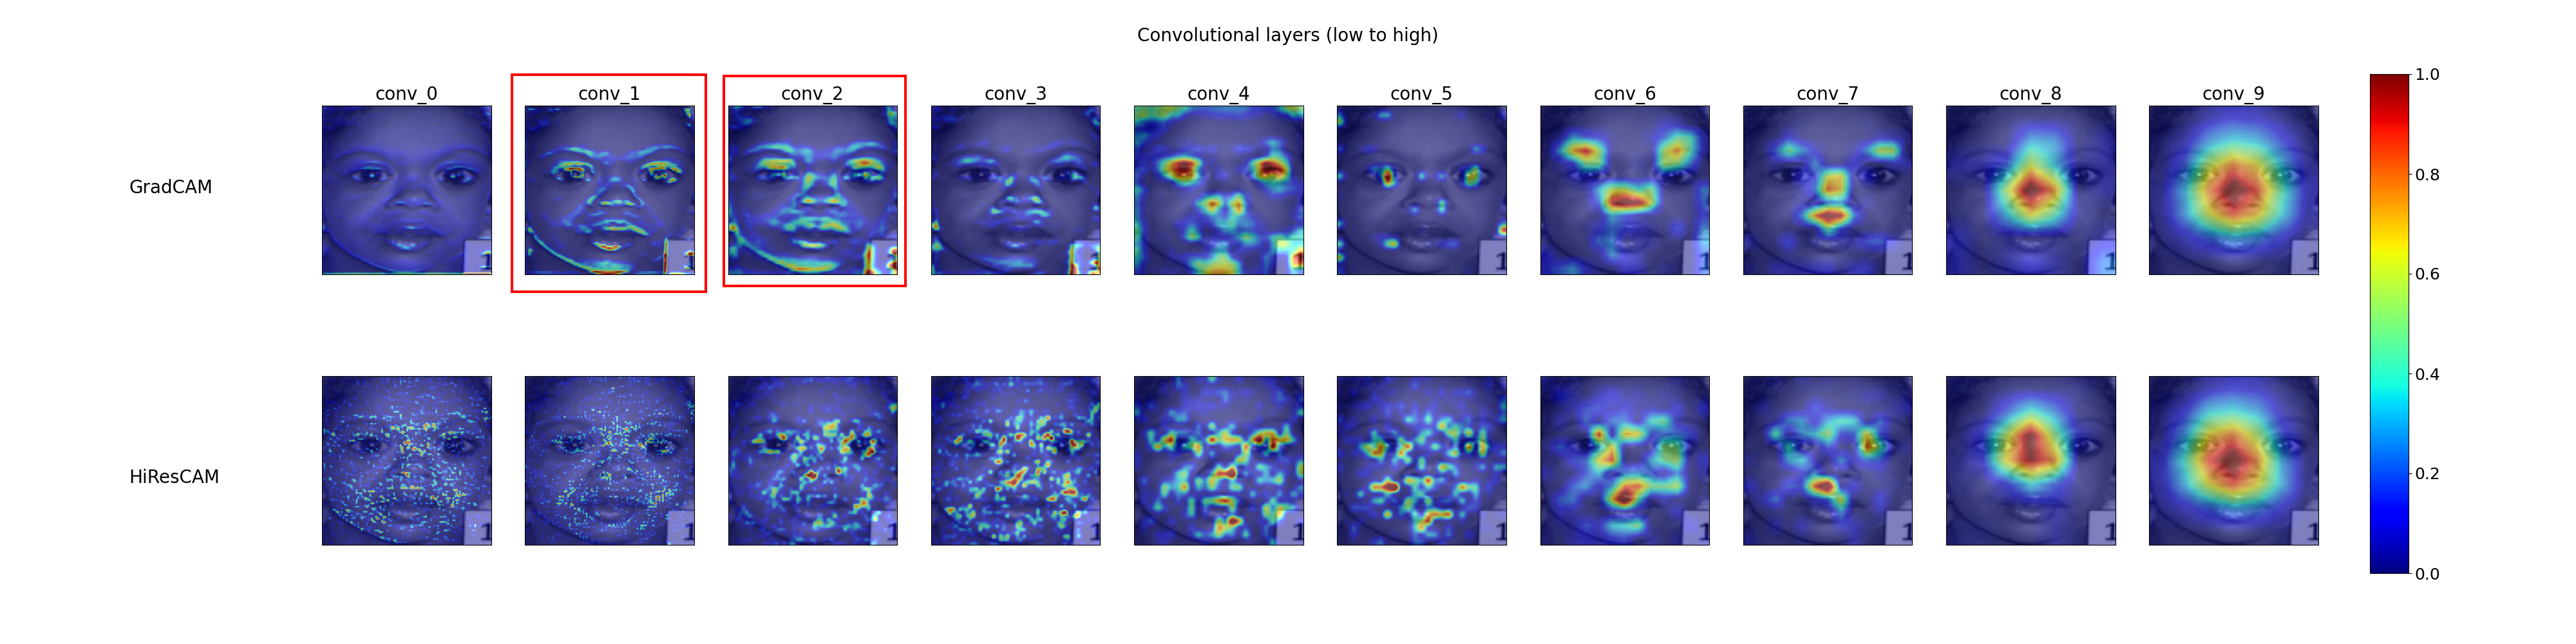
\includegraphics[scale=0.22, trim = 1cm 2.50cm 1cm 2.50cm, clip]{chapter6/william/2_137_layer.png}
    	\caption[Example layer-wise activation map visualizations for instances presented in the questionnaire]{Example layer-wise activation map visualizations for instances presented in the questionnaire. Layers highlighting syndromic features are boxed in red.}
	   \label{fig_layer_quest}	
    \end{sidewaysfigure}

	\begin{sidewaysfigure}
		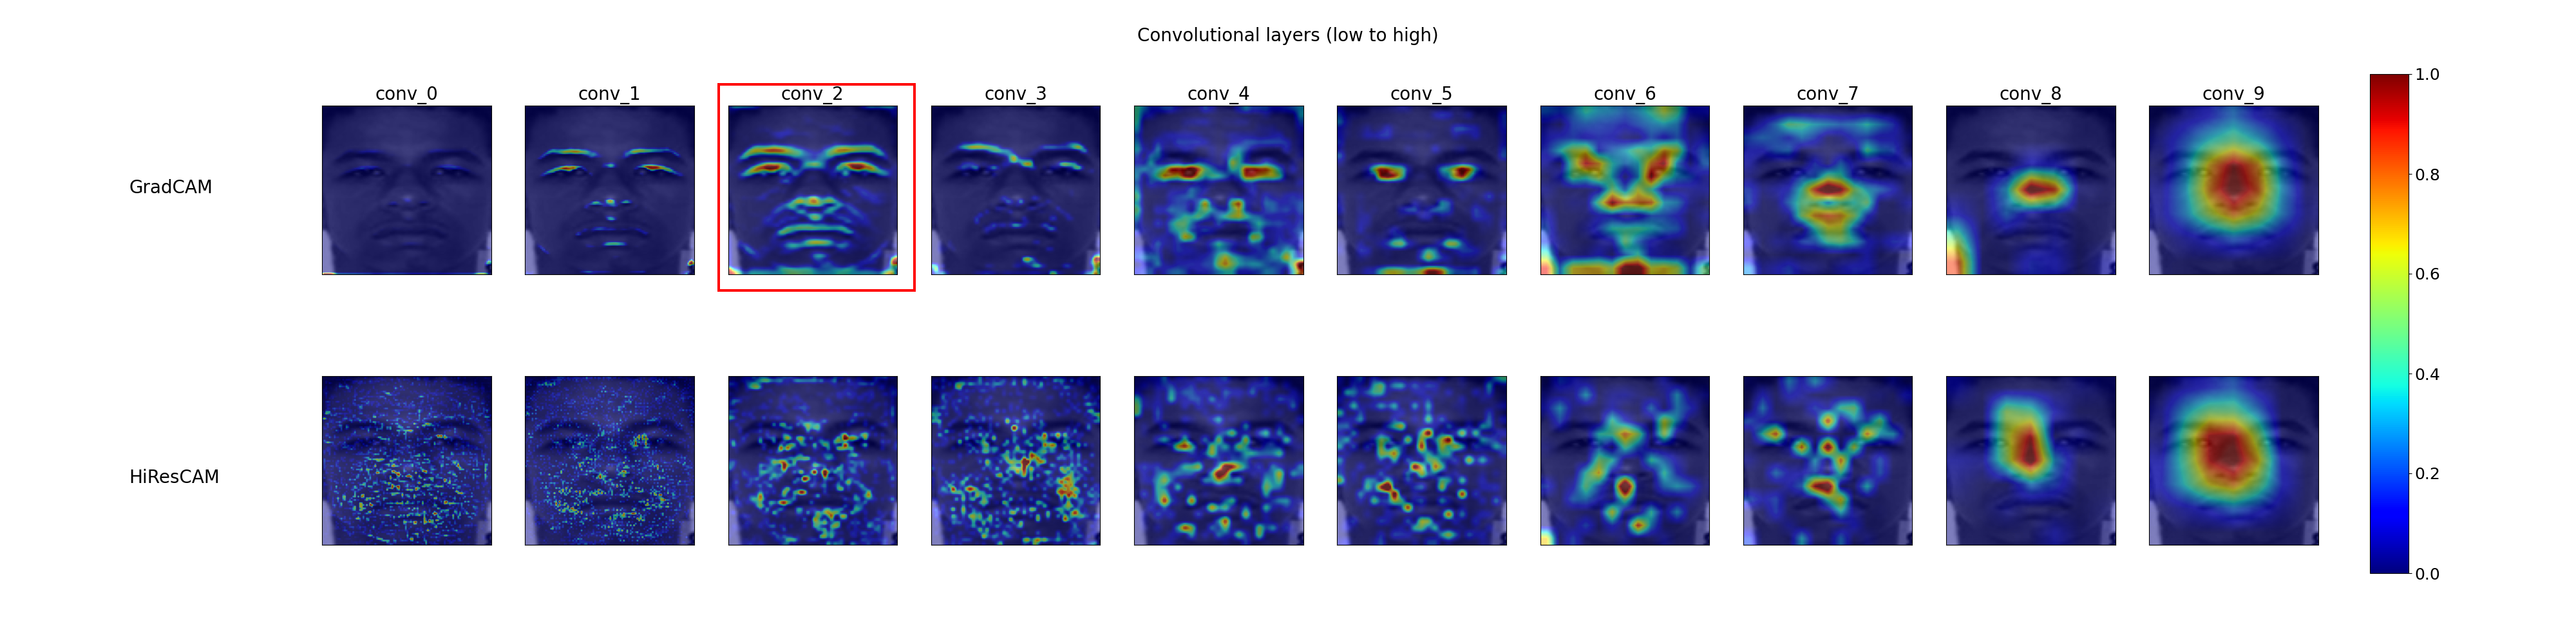
\includegraphics[scale=0.22, trim = 1cm 2.50cm 1cm 2.50cm, clip]{chapter6/william/20_95_layer.png}		
		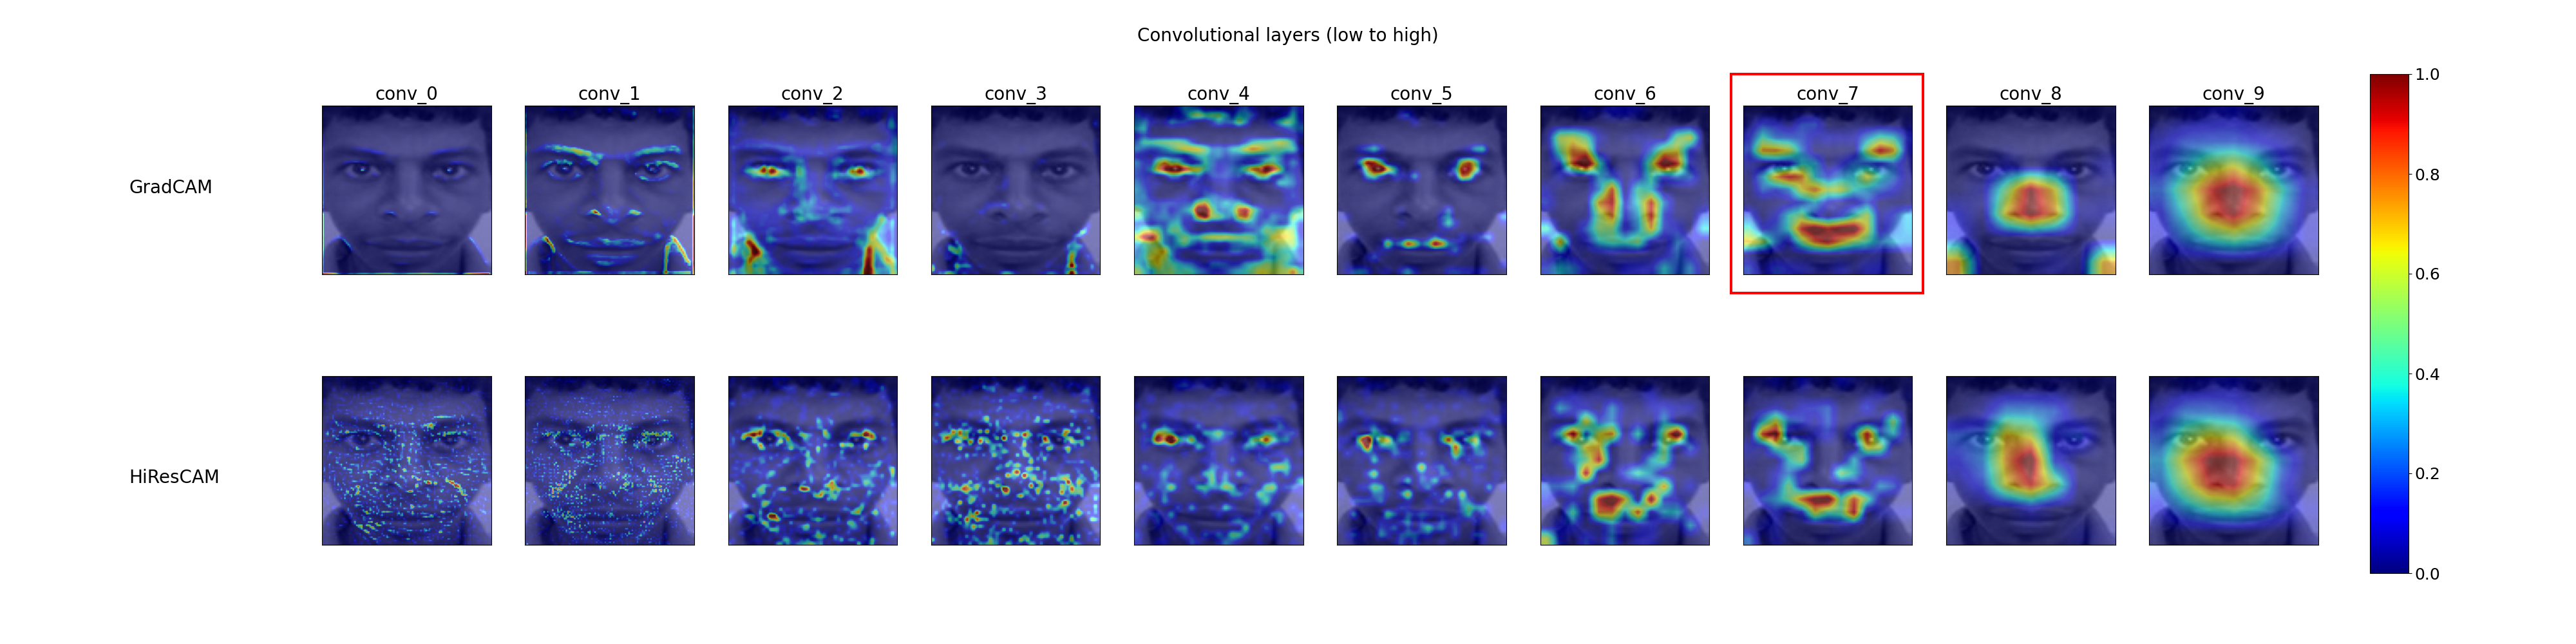
\includegraphics[scale=0.22, trim = 1cm 2.50cm 1cm 2.50cm, clip]{chapter6/william/16_3632_layer.png}
		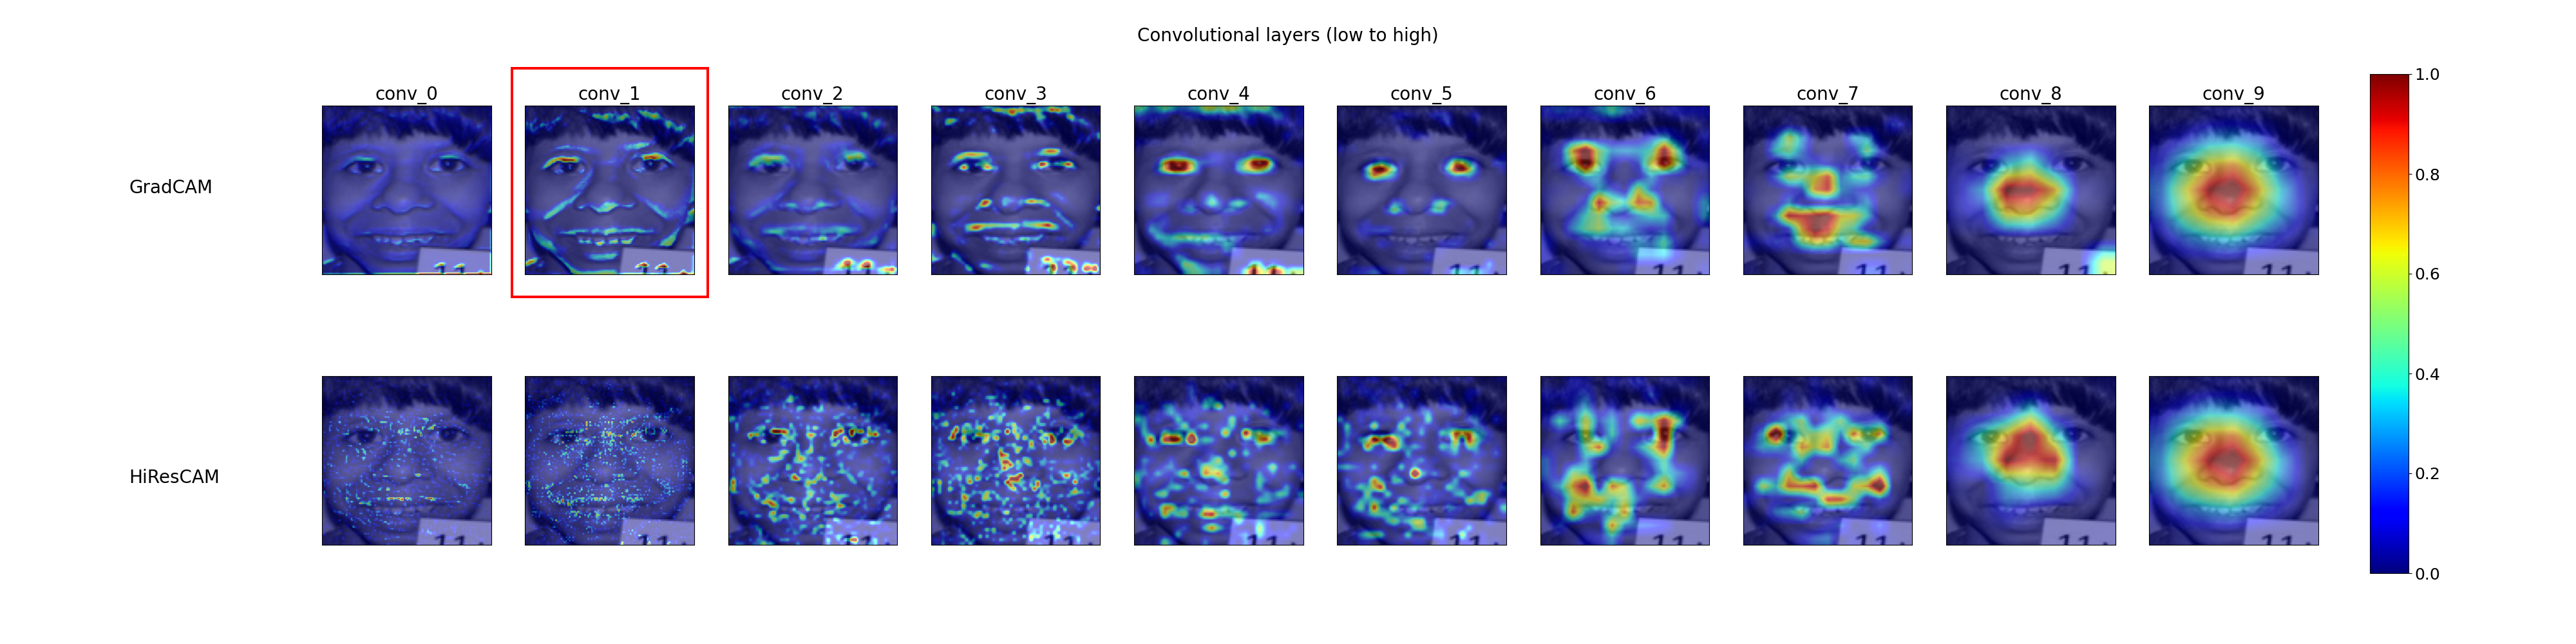
\includegraphics[scale=0.22, trim = 1cm 2.50cm 1cm 2.50cm, clip]{chapter6/william/14_142_layer.png}
		\caption[Example layer-wise activation map visualizations for instances not present in the questionnaire but in GMDB dataset]{Example layer-wise activation map visualizations for instances not present in the questionnaire but in GMDB dataset. Layers highlighting syndromic features are boxed in red.}
		\label{fig_layer_gmdb}
	\end{sidewaysfigure}
    \pagebreak
    
    \section{Experiment B. Composite Face Generation}
    \noindent
    A composite face provides a characteristic representation of the facial phenotype of a given genetic
    syndrome. Figure \ref{fig_comp_gmdb} contains composite faces of the twelve largest classes of the GMDB dataset. 
       \begin{figure}[H]
    	\begin{subfigure}[t]{0.45\textwidth}
    		\centering
    		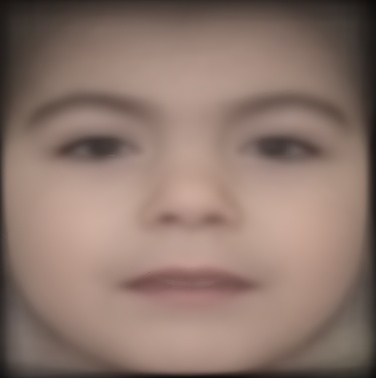
\includegraphics[scale=0.4]{chapter6/cfaces/0.jpg}
    		\caption{Cornelia de Lange syndrome}    		
    	\end{subfigure}
    	\begin{subfigure}[t]{0.45\textwidth}
    		\centering
    		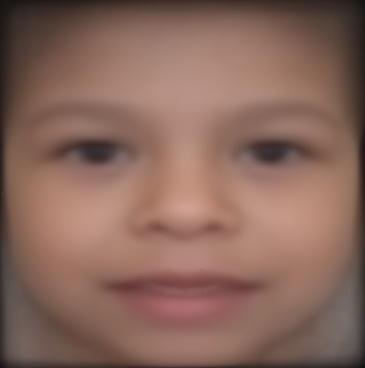
\includegraphics[scale=0.4]{chapter6/cfaces/1.jpg}
    		\caption{Williams syndrome}   		
    	\end{subfigure}
    	\begin{subfigure}[t]{0.45\textwidth}
    		\centering
    		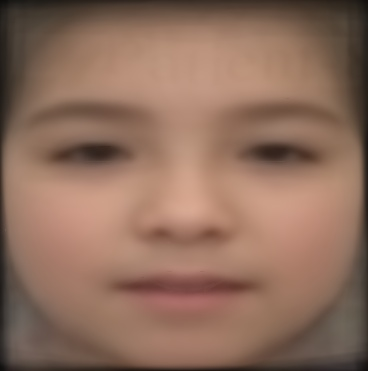
\includegraphics[scale=0.4]{chapter6/cfaces/2.jpg}
    		\caption{Wiedemann-Steiner syndrome}    	
    	\end{subfigure}
    \begin{subfigure}[t]{0.45\textwidth}
    	\centering
    	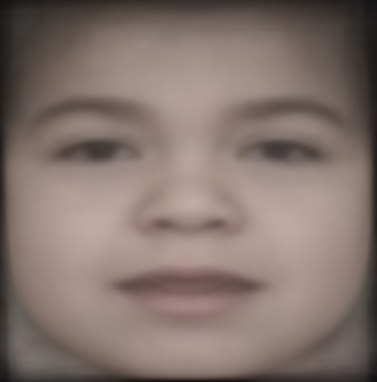
\includegraphics[scale=0.4]{chapter6/cfaces/3.jpg}
    	\caption{Mucopolysaccharidoses}
    \end{subfigure}
	\begin{subfigure}[t]{0.45\textwidth}
		\centering
		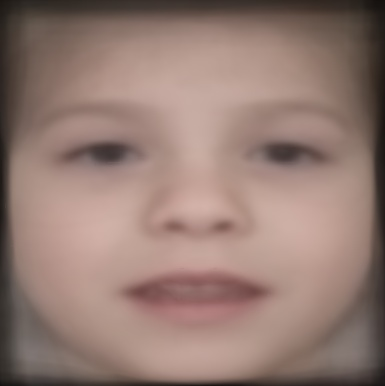
\includegraphics[scale=0.4]{chapter6/cfaces/4.jpg}
		\caption{Nicolaides-Baraitser syndrome}
	\end{subfigure}
	\hspace{1.5cm}
	\begin{subfigure}[t]{0.45\textwidth}
		\centering
		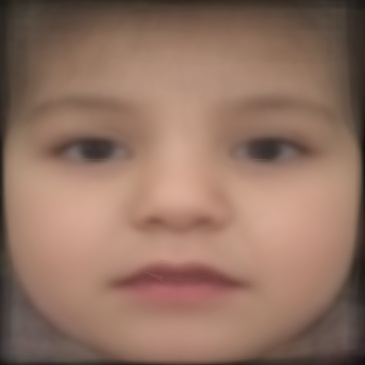
\includegraphics[scale=0.4]{chapter6/cfaces/5.jpg}
		\caption{Hyperphosphatasia with mental retardation syndrome}
	\end{subfigure}
	\end{figure}
	\begin{figure}[H]\continuedfloat
		\begin{subfigure}[t]{0.45\textwidth}
			\centering
			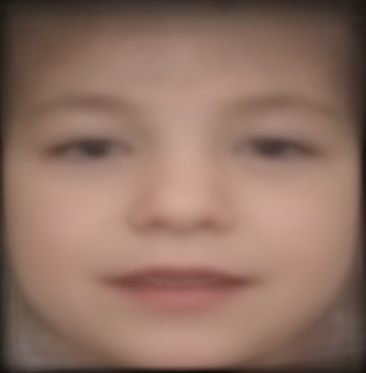
\includegraphics[scale=0.4]{chapter6/cfaces/6.jpg}
			\caption{Baraitser-Winter syndrome}
		\end{subfigure}
		\begin{subfigure}[t]{0.45\textwidth}
			\centering
			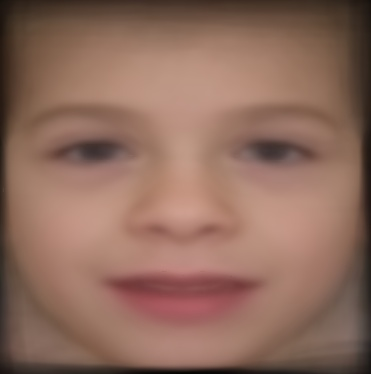
\includegraphics[scale=0.4]{chapter6/cfaces/7.jpg}
			\caption{Smith-Lemli-Opitz syndrome}
		\end{subfigure}
		\begin{subfigure}[t]{0.45\textwidth}
			\centering
			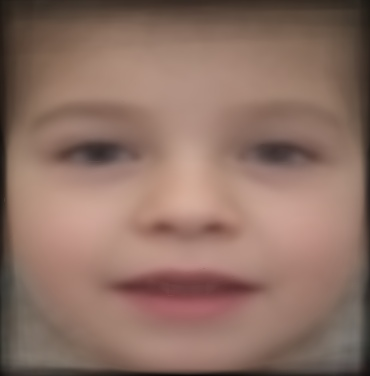
\includegraphics[scale=0.4]{chapter6/cfaces/8.jpg}
			\caption{Coffin-Siris syndrome}
		\end{subfigure}
		\hspace{1.5cm}
		\begin{subfigure}[t]{0.45\textwidth}
			\centering
			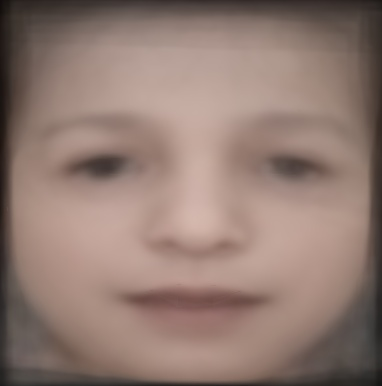
\includegraphics[scale=0.4]{chapter6/cfaces/9.jpg}
			\caption{Treacher Collins syndrome}
		\end{subfigure}
			\begin{subfigure}[t]{0.45\textwidth}
		\centering
		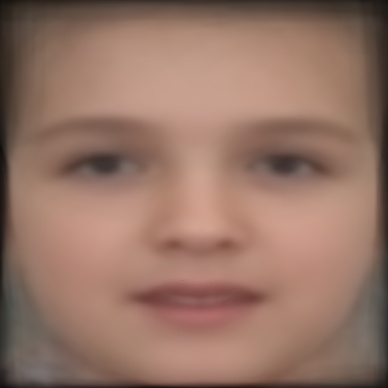
\includegraphics[scale=0.4]{chapter6/cfaces/10.jpg}
		\caption{Sotos syndrome}
	\end{subfigure}
	\hspace{1.5cm}
	\begin{subfigure}[t]{0.45\textwidth}
		\centering
		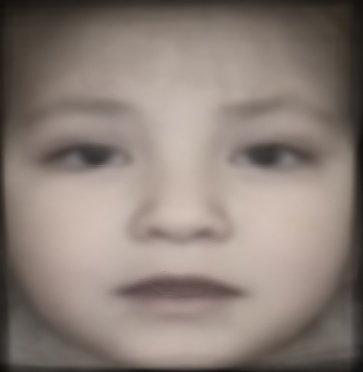
\includegraphics[scale=0.4]{chapter6/cfaces/11.jpg}
		\caption{Kabuki syndrome}
	\end{subfigure}
	\caption{Composite faces of the twelve largest syndrome classes in GMDB dataset}
	\label{fig_comp_gmdb}
\end{figure}

\begin{figure}[H]
	\centering
	\begin{subfigure}[t]{0.8\textwidth}
		\centering
		\hspace{-0.5cm}
		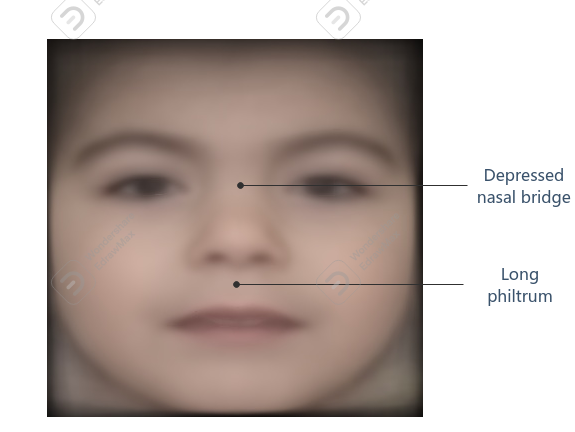
\includegraphics[scale=0.53]{chapter6/cfaces/0_labeled.png}
		\caption{Composite face of CDLS labeled with phenotypic features}
	\end{subfigure}
	\begin{subfigure}[t]{0.8\textwidth}
		\centering
		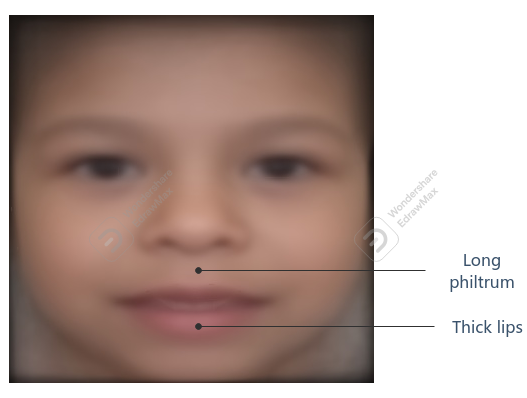
\includegraphics[scale=0.53]{chapter6/cfaces/1_labeled.png}
		\caption{Composite face of WBS labeled with phenotypic features}
	\end{subfigure}
	\begin{subfigure}[t]{0.8\textwidth}
		\centering
		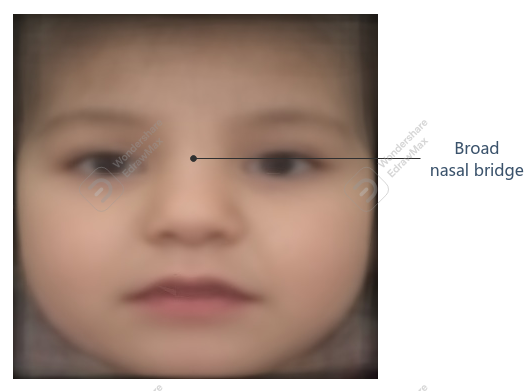
\includegraphics[scale=0.53]{chapter6/cfaces/5_labeled.png}
		\caption{Composite face of HPMRS labeled with feature}
		\label{sfig_diff_3}
	\end{subfigure}
	\caption{Composite faces of the syndromes evaluated by the clinician labeled with phenotypic features}
	\label{fig_comp_lab}
\end{figure}
The clinician evaluated composite faces representing six syndromes similar to other experimental artifacts. He found all three faces pertaining to the syndromes he specialized (CDLS, WBS, HPMRS) to contain their respective characteristic features. The same was reported for SMOS, although he was not experienced in diagnosing the syndrome. We observed a few though not all distinctive facial features in composite faces of CDLS, WBS and HPMRS (refer to Figure \ref{fig_comp_lab}). The absence of other characteristic features can be attributed to the fact that averaging variations in their constituent images generated composite faces. Besides acting as an input artifact for syndrome-wise attribution map generation, composite faces can serve as reference images for clinicians.

  	\section{Experiment C. Syndrome-wise Attribution Map Generation} \label{sec_expc}
  	\noindent
    The clinician evaluated four out of six syndrome-wise attribution maps presented to him representing CDLS, WBS, HPMRS, and CSS (refer to figures \ref{fig_synd_map_1} and \ref{fig_synd_map_2}). The following could be deduced from his responses and by analyzing the maps:
    \begin{itemize}
    	\item The composite face-GradCAM and average attribution-GradCAM combinations were chosen to best highlight the characteristic feature of CDLS. For example, it can be observed from Figure \ref{fig_synd_map_1} that the occurrence of synophrys is featured in both the maps.
    	\item In the case of WBS, representations generated using composite face-FullGrad and average attribution-FullGrad pairs were preferred over other options. Both the attribution maps marked the depressed nasal bridge feature of the syndrome (refer to Figure \ref{fig_synd_map_1}).
    	\item The clinician considered composite face-GradCAM and average attribution-GradCAM combinations to closely represent the broad nasal bridge and hypertelorism features associated with HPMRS (refer to Figure \ref{fig_synd_map_2}).
    	\item Unlike the above discussed syndrome-wise maps, down-slanting palpebral fissures, a feature in the eye region was highlighted in the composite face-CustomGradCAM and average attribution-CustomGradCAM maps of CSS (refer Figure \ref{fig_synd_map_2}). This led the clinician to pick them over others.
    	\item Maps generated using the SVD approach were not useful in any of the evaluations. In addition, we found the approach to produce maps in which the image background was highlighted (refer to Figure \ref{fig_synd_map_1}).
    \end{itemize}
	In general, the syndrome-wise attribution maps produced from average attribution-GradCAM and average attribution-FullGrad combinations successfully highlighted the most characteristic feature of respective syndromes. However, similar to the case of patient-wise attribution maps, most of the maps highlighted the nasal region, except for CSS.  
    \pagebreak	
    
    \clearpage
        \begin{sidewaysfigure}
    	\includegraphics[scale=0.5]{chapter6/syndrome_maps/0.png}
    	
    	\includegraphics[scale=0.5]{chapter6/syndrome_maps/1.png}
    	
    	\caption[Syndrome-wise attribution maps of CDLS and WBS]{Syndrome-wise attribution maps of CDLS (top three rows) and WBS (bottom three rows). Options chosen by the clinician are boxed in black.}
    	\label{fig_synd_map_1}	
    	\end{sidewaysfigure}
    
            \begin{sidewaysfigure}
    	\includegraphics[scale=0.5]{chapter6/syndrome_maps/5.png}
    	    	\includegraphics[scale=0.5]{chapter6/syndrome_maps/8.png}
    	
    	\caption[Syndrome-wise attribution maps of HPMRS and CSS]{Syndrome-wise attribution maps of HPMRS (top three rows) and CSS (bottom three rows). Options chosen by the clinician are boxed in black.}
    	\label{fig_synd_map_2}	
    \end{sidewaysfigure}
    \clearpage
	\section{Experiment D. Dataset Imbalance - Explanation Quality Analysis}
	\noindent
	 Unlike other experiments, analysis of this experiment's artifacts was done without the help of a clinician. Most of the changes observed in the attribution maps of the above-listed classifiers couldn't be interpreted in a meaningful way. Therefore, in this a qualitative analysis of some important observations is provided. For comparison, we used corresponding attribution maps generated using the 139-class GestaltMatcher classifier model (GM) as the baseline.
	 	
	\begin{itemize}
	
			
		\item Figure \ref{fig_cdls_imb} contains attribution maps of a CDLS patient image generated from the set of classifier models considered for this experiment (a-d) and the GM model. It can be observed that the regions highlighted in FullGrad maps remain unchanged in all cases. However, attention regions of GradCAM and HiResCAM maps differ for every model.
				
		\item It can be observed that the attention region of GC1, the syndrome vs. healthy classifier, has a wider region of attention than the GM model. Also, their regions of attention differ from each other. GC1 focused more on the right cheek region, while GM focused on the labella (the meeting point of eyebrows), which is characteristic to CDLS. Attention regions of GC2 were observed to be narrower than that of GC1. \enquote {No significant changes were observed between attribution maps GC3 and GC4, the classifiers trained on balanced and imbalanced sets of classes respectively}.
		
		\item Attribution maps shown in Figure \ref{fig_gm_wearables} reveal that except GM, all other classifier models get affected by the presence of spectacles on the patient's face. The GM model focuses on the distinct eyebrow region (refer to Figure \ref{fig_wearable_gm}).
		
		\item Attribution maps of healthy faces produced using GC1 reveal that the model uses the same set of features to recognize images of both classes. This indicates that the neural network model looks for the presence or absence of certain discriminative features in an image to classify the same. For example, it can be observed from visualizations in Figure \ref{fig_health_syn_exam} that the nasal region was used to recognize both the healthy and syndromic images.
		\end{itemize}
	
		\begin{figure}[H]
		\begin{subfigure}[t]{1\textwidth}
			\centering
			\includegraphics[width=\textwidth, trim = 1cm 2.50cm 1cm 2cm, clip]{chapter6/xai_imb/0n_gm.png}
			\caption{GC1}
			\label{fig_cdls_imb_a}
		\end{subfigure}
			\begin{subfigure}[t]{1\textwidth}
			\centering
			\includegraphics[width=\textwidth, trim = 1cm 2.50cm 1cm 2cm, clip]{chapter6/xai_imb/01_gm.png}
			\caption{GC2}
			\label{fig_cdls_imb_b}
		\end{subfigure}
			\begin{subfigure}[t]{1\textwidth}
			\centering
			\includegraphics[width=\textwidth, trim = 1cm 2.50cm 1cm 2cm, clip]{chapter6/xai_imb/b_gm.png}
			\caption{GC3}
			\label{fig_cdls_imb_c}
		\end{subfigure}
			\begin{subfigure}[t]{1\textwidth}
			\centering
			\includegraphics[width=\textwidth, trim = 1cm 2.50cm 1cm 2cm, clip]{chapter6/xai_imb/i_gm.png}
			\caption{GC4}
			\label{fig_cdls_imb_d}
		\end{subfigure}
			\begin{subfigure}[t]{1\textwidth}
			\centering
			\includegraphics[width=\textwidth, trim = 1cm 2.50cm 1cm 2cm, clip]{chapter6/xai_imb/0_gm.png}
			\caption{GM}
			\label{fig_cdls_imb_e}
		\end{subfigure}
	\caption[Attribution maps of a CDLS patient image generated using different classifier models]{Attribution maps of a CDLS patient image generated using different classifier models. Meaningful changes in regions of attention are marked with a black bounding box.}
	\label{fig_cdls_imb}
	\end{figure}
	
\begin{figure}[H]
	\begin{subfigure}[t]{1\textwidth}
		\centering
		\includegraphics[width=\textwidth, trim = 1cm 2.50cm 1cm 2cm, clip]{chapter6/xai_imb/wearables/0n.png}
		\caption{GC1}
	\end{subfigure}
	\begin{subfigure}[t]{1\textwidth}
		\centering
		\includegraphics[width=\textwidth, trim = 1cm 2.50cm 1cm 2cm, clip]{chapter6/xai_imb/wearables/01.png}
		\caption{GC2}
	\end{subfigure}
	\begin{subfigure}[t]{1\textwidth}
		\centering
		\includegraphics[width=\textwidth, trim = 1cm 2.50cm 1cm 2cm, clip]{chapter6/xai_imb/wearables/i.png}
		\caption{GC3}
		
	\end{subfigure}
	\begin{subfigure}[t]{1\textwidth}
		\centering
		\includegraphics[width=\textwidth, trim = 1cm 2.50cm 1cm 2cm, clip]{chapter6/xai_imb/wearables/b.png}
		\caption{GC4}
	\end{subfigure}
	\begin{subfigure}[t]{1\textwidth}
		\centering
		\includegraphics[width=\textwidth, trim = 1cm 2.50cm 1cm 2cm, clip]{chapter6/xai_imb/wearables/gm.png}
		\caption{GM}
		\label{fig_wearable_gm}
	\end{subfigure}
	\caption{Attribution maps depicting the effect of wearables on attention of different classifier models}
	\label{fig_gm_wearables}
\end{figure}

\begin{figure}[H]
	\begin{subfigure}[t]{1\textwidth}
		\centering
		\includegraphics[width=\textwidth, trim = 1cm 2.50cm 1cm 2cm, clip]{chapter6/xai_imb/health_1.png}
		\caption{An example of correctly classified healthy face}
		
	\end{subfigure}
	\begin{subfigure}[t]{1\textwidth}
		\centering
		\includegraphics[width=\textwidth, trim = 1cm 2.50cm 1cm 2cm, clip]{chapter6/xai_imb/health_2.png}
		\caption{An example of correctly classified healthy face}
		
	\end{subfigure}
	\begin{subfigure}[t]{1\textwidth}
		\centering
		\includegraphics[width=\textwidth, trim = 1cm 2.50cm 1cm 2cm, clip]{chapter6/xai_imb/synd_exam.png}
		\caption{An example of correctly classified CDLS face}
	\end{subfigure}
	\caption{Attribution maps of healthy and syndromic facial images}
	\label{fig_health_syn_exam}
\end{figure}
	\section{Summary of Results}
	This section summarizes results presented earlier in this chapter:
	\begin{itemize}
		\item Experiment A: Patient-wise attribution maps representing six genetic syndromes were evaluated by an experienced clinical geneticist. We considered his responses related to three of the six syndromes he was familiar, for our analyses (CDLS, WBS, and HPMRS). Attribution maps generated using the FullGrad method were voted to highlight relevant facial features in the majority of samples, representing CDLS and HPMRS classes. None of the presented maps highlighted \enquote{thick lips}, the characteristic feature of WBS. Layer-wise activation visualization revealed that the missing feature gets highlighted in maps of convolutional layers different from the ones considered earlier. Extending the analysis to other samples showed that maps of different layers contained highlighted key feature regions for different instances.
		\item Experiment B: Results from the clinician's evaluation of composite faces were presented. The expert was convinced that CDLS, WBS, HPMRS and SMOS composite faces represented their respective syndromes. Besides, it was reported that they contained one or two, but not all, characteristic features of their related syndromes. Therefore, faces of CDLS, WBS and HPMRS labeled with the identified features were presented, along with the ones representing other nine syndromes in GMDB dataset.
		\item Experiment C: The clinician evaluated four syndrome-wise attribution maps representing CDLS, WBS, HPMRS, and CSS. The composite face-average attribution combination was picked to better highlight key regions of CDLS and HPMRS. The composite face-FullGrad and average attribution-FullGrad maps closely matched the clinician's region of attention for WBS. Downslanting palpebral fissures, a characteristic feature of CSS was contained in the regions highlighted by composite face - customGradCAM and average attribution-custom GradCAM maps. Maps generated using the SVD approach were not found to be helpful.
		\item Experiment D:  No significant effects of dataset imbalance were observed in attribution maps. Results of the experiment show that the classifier model trained to differentiate CDLS faces from healthy faces relies on features of the same facial region to classify input into either of the two. In addition, it was found that the GestaltMatcher classifier model's attention to critical features, is not affected by the presence of wearables like spectacles in the facial image.
	\end{itemize}
    \section{Inferences}\label{sec_inf}
    In this section, inferences drawn from the results of conducted experiments are presented.  
    \begin{itemize}
    	\item \textbf{1. Nasal profile,  a discriminative feature for syndrome recognition:} We observed the nose region to be highlighted in attribution maps generated for samples of many other classes, which were not represented in the questionnaire. Figure \ref{fig_nose_region} contains some examples of such instances. The recurrent behavior of the attribution methods to highlight the nose region may indicate the facial region's distinctiveness and importance in the diagnosis of rare genetic conditions. In order to verify this hypothesis, we looked into Online Mendelian Inheritance in Man (OMIM\footnotetext[1]{\url{https://www.omim.org}}), an online compendium of human genes and phenotypes. We searched for facial features linked to syndromes of the ten largest classes of GMDB (Refer Table \ref{tab_nose_gmdb}). We found eight out of the ten syndromes to be linked to at least feature in the nose region. This finding supports our hypothesis and could possibly help the scientific community in discovering new gene-phenotype associations. 
    	
    	\begin{table}[H]
    		\centering
    		\begin{tabular}{|c|l|}
    			\hline
    			\textbf{Syndrome}                                                                               & \multicolumn{1}{c|}{\textbf{Features in the nose region}}                                                                                              \\ \hline
    			Cornelia de Lange syndrome I                                                                    & Anteverted nostrils,  depressed nasal bridge                                                                                                           \\ \hline
    			Williams syndrome                                                                               & Anteverted nares, depressed nasal bridge                                                                                                               \\ \hline
    			Wiedemann-Steiner syndrome                                                                      & Broad nose, wide nasal bridge, depressed nasal tip                                                                                                     \\ \hline
    			Mucopolysaccharidoses                                                                           & None                                                                                                                                                   \\ \hline
    			Nicolaides-Baraitser syndrome                                                                   & \begin{tabular}[c]{@{}l@{}}Narrow nasal bridge, Broad nasal base, \\ upturned nasal tip, thick alae nasi, anteverted nares\end{tabular}                \\ \hline
    			\begin{tabular}[c]{@{}c@{}}Hyperphosphatasia with \\ mental retardation syndrome I\end{tabular} & \begin{tabular}[c]{@{}l@{}}Broad nasal bridge, broad nasal tip,\\ short nose\end{tabular}                                                              \\ \hline
    			Baraitser-Winter syndrome                                                                       & \begin{tabular}[c]{@{}l@{}}Broad nasal bridge, broad nasal tip, short nose,\\ large, squared nose tip, \\ prominent nasal root on profile\end{tabular} \\ \hline
    			Smith-Lemli-Opitz syndrome                                                                      & Anterverted nares, broad and flat nasal bridge                                                                                                         \\ \hline
    			Coffin-Siris syndrome I                                                                         & Broad nasal tip                                                                                                                                        \\ \hline
    			Treacher Collins syndrome I                                                                     & None                                                                                                                                                   \\ \hline
    		\end{tabular}
    		\caption{Features in the nose region associated with the ten largest classes of GMDB dataset. Source: OMIM}
    		\label{tab_nose_gmdb}
    	\end{table}
    	\item{\textbf{2. Attribution methods are limited by their expressiveness}:} Attribution methods highlight the regions that were significant for a particular prediction by a neural network. Although attribution maps help localize a network's attention regions, they cannot provide the context of the explanation. In the case of this research work, the nose region gets highlighted in most of the syndromes' attribution maps. However, we cannot to deduce what particular feature attributes are used by GestaltMatcher for its predictions, for example, symmetry or shape profile of the nose. This could be determined using other XAI techniques such as feature and concept visualizations (refer Section \ref{sec_nn_methods}).
    	
    	\item{\textbf{3. All explanations do not carry a real-world meaning:}} Each XAI method considered in this work approaches the problem of attribution in its way. GradCAM converts the problem into \enquote{weakly supervised localization} and aims to localize the target class in form of an object. This proves helpful when classes represent real-world objects which have a well-defined physical form. In our case, the target categories represent genetic syndromes, entities characterized by distinct features, but dont exist as individual objects.\\ 
    	HiResCAM, a more faithful approach avoids the gradient-averaging step to reveal all attention regions of a neural network model. It can be inferred from the clinician's evaluation that unfiltered explanations produced by the method were not chosen to highlight the facial features that are considered important for diagnosis by humans. This is possible because the GestaltMatcher model focuses on multiple sparse sections of a facial image whose composition does not correspond to a feature of a given syndrome. The success of the FullGrad approach can be attributed to its layer-agnostic nature and ability to consolidate input and neuronal attributions into a single representation.
    	
    	\item{\textbf{4. XAI methods are not ready for high-stake applications:}}  One of the primary objectives of this research work is to explain the rationale behind predictions of GestaltMatcher, and inturn make the model transparent, so that it can be used in a clinical setting. The results of the conducted experiments show that the model used certain facial features known to the medical community for making predictions. However, in many instances, the classifier model either relied on the same set of features or sparsely focused on regions whose composition did not carry a real-world meaning. Besides, the inconsistency in layers that highlighted key features also posed a challenge in explaining the model's predictions. Therefore, we feel the need for improvements in XAI methods before they are deployed to explain predictions of neural network models used for high stake applications like genetic syndrome diagnosis. However, as of now, they make an excellent tool for \enquote{knowledge discovery}.
    \end{itemize} 
		\begin{figure}[H]
		\centering			
		\begin{subfigure}[t]{1\textwidth}
			\centering
			\includegraphics[width=\textwidth, trim = 1cm 2.50cm 1cm 2cm, clip]{chapter6/2_nose.png}
			\caption{Widemann-Steiner syndrome}	
		\end{subfigure}
		\begin{subfigure}[t]{1\textwidth}
			\centering
			\includegraphics[width=\textwidth, trim = 1cm 2.50cm 1cm 2cm, clip]{chapter6/3_nose.png}
			\caption{Mucopolysaccharidoses}
		\end{subfigure}
		\begin{subfigure}[t]{1\textwidth}
			\centering
			\includegraphics[width=\textwidth, trim = 1cm 2.50cm 1cm 2cm, clip]{chapter6/6_nose.png}
			\caption{Baraitser-Winter syndrome}
		\end{subfigure}
%		\begin{subfigure}[t]{1\textwidth}
%		\centering
%		\includegraphics[width=\textwidth, trim = 1cm 2.50cm 1cm 2cm, clip]{chapter6/9_nose.png}
%		\caption{Treacher Collins syndrome}
%		\end{subfigure}
		\caption{Samples from other syndromes with their attribution maps highlighting the nasal region}
		\label{fig_nose_region}
		\end{figure}

\end{document}
